What is the gradient at $r_1$? What value of $\sigma$ should you use so that $\lambda_1$ and $r_2$ are reasonable? Plot $r_2$ on your contour plot.

\begin{solution}
\begin{align*}
    \nabla f(r_1) &= \begin{bmatrix}
        -3.9 \\ 0.3
    \end{bmatrix}
\end{align*}

With a $\sigma$ value of 0.9, the $\lambda_1$ value is 0.09. This results in the following $r_2$ vector.

\begin{center}
    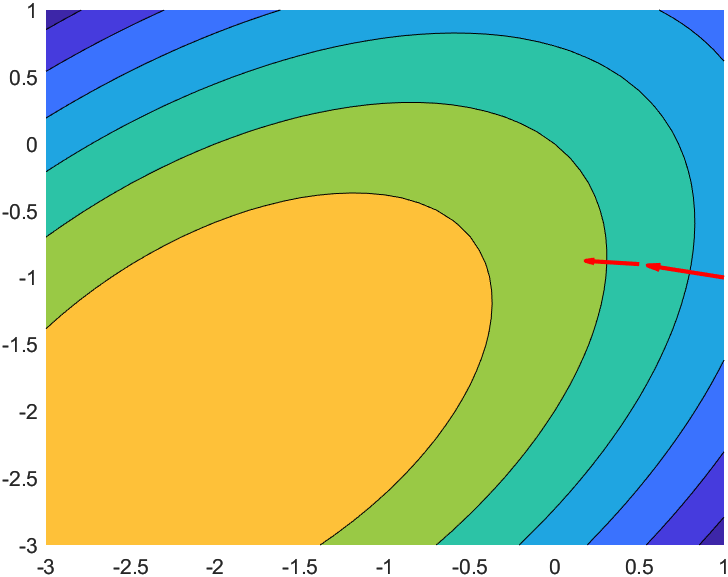
\includegraphics[width=0.5\textwidth]{img/e7p7.png}
\end{center}
\end{solution}